	%Câu 13
	\begin{ex}%[2D4N3-3]
		Gọi $V$ là thể tích của khối tròn xoay thu được khi quay hình thang cong, giới hạn bởi đồ thị hàm số $y=\sin x$, trục $Ox$, trục $Oy$ và đường thẳng $x=\dfrac{\pi}{2}$, xung quanh trục $Ox$. Mệnh đề nào dưới đây đúng?
		\choice
		{$V=\displaystyle\int\limits_0^{\tfrac{\pi}{2}}{\sin^2x\mathrm{\,d}x}$}
		{$V=\displaystyle\int\limits_0^{\tfrac{\pi}{2}}{\sin x\mathrm{\,d}x}$}
		{\True $V=\pi\displaystyle\int\limits_0^{\tfrac{\pi}{2}}{\sin^2x\mathrm{\,d}x}$}
		{$V=\pi\displaystyle\int\limits_0^{\tfrac{\pi}{2}}{\sin x\mathrm{\,d}x}$}
		\loigiai{
			Công thức tính $V=\pi\displaystyle\int\limits_a^b{f^2(x)\mathrm{\,d}x}$.
		}
	\end{ex}

	%Câu 14
	\begin{ex}%[2D4H3-3]
		Thể tích khối tròn xoay được sinh ra khi quay hình phẳng giới hạn bởi đồ thị của hàm số $y=x^2-2x$, trục hoành, đường thẳng $x=0$ và $x=1$ quanh trục hoành bằng
		\choice
		{$\dfrac{16\pi}{15}$}
		{$\dfrac{2\pi}{3}$}
		{$\dfrac{4\pi}{3}$}
		{\True $\dfrac{8\pi}{15}$}
		\loigiai{
			Ta có
			\allowdisplaybreaks
			\begin{eqnarray*}
				V&=&\pi\displaystyle\int\limits_0^1\left(x^2-2x\right)^2\mathrm{\,d}x\\
				&=&\pi\displaystyle\int\limits_0^1\left(x^4-4x^3+4x^2\right)\mathrm{\,d}x\\
				&=&\pi \cdot \left(\dfrac{x^5}{5}-x^4+\dfrac{4x^3}{3}\right)\Bigg|_0^1\\
				&=&\pi \cdot \left(\dfrac{1}{5}-1+\dfrac{4}{3}\right)=\dfrac{8\pi}{15}.
			\end{eqnarray*}
			}
	\end{ex}

	%Câu 15
	\begin{ex}%[2D4N3-3]
		Cho miền phẳng $(D)$ giới hạn bởi $y=\sqrt x$, hai đường thẳng $x=1$, $x=2$ và trục hoành. Tính thể tích khối tròn xoay tạo thành khi quay $(D)$ quanh trục hoành.
		\choice
		{$3\pi $}
		{\True $\dfrac{3\pi}{2}$}
		{$\dfrac{2\pi}{3}$}
		{$\dfrac{3}{2}$}
		\loigiai{
			$V=\pi\displaystyle\int\limits_1^2x\mathrm{\,d}x=\dfrac{\pi x^2}{2}\Bigg|_1^2=\dfrac{3\pi}{2}$.
			}
	\end{ex}
	
	%Câu 16
	\begin{ex}%[2D4N3-3]
		Cho hình phẳng $(H)$ giới hạn bởi các đường $y=2x-x^2$, $y=0$. Quay $(H)$ quanh trục hoành tạo thành khối tròn xoay có thể tích là
		\choice
		{$\displaystyle\int\limits_0^2\left(2x-x^2\right)\mathrm{\,d}x$}
		{\True $\pi\displaystyle\int\limits_0^2\left(2x-x^2\right)^2\mathrm{\,d}x$}
		{$\displaystyle\int\limits_0^2\left(2x-x^2\right)^2\mathrm{\,d}x$}
		{$\pi\displaystyle\int\limits_0^2\left(2x-x^2\right)\mathrm{\,d}x$}
		\loigiai{
			Theo công thức ta chọn $V=\pi\displaystyle\int\limits_0^2\left(2x-x^2\right)^2\mathrm{\,d}x$.
			}
	\end{ex}
	
	%Câu 17
	\begin{ex}%[2D4H3-3]
		Cho hình phẳng giới hạn bởi các đường $y=\sqrt{x}-2$, $y=0$ và $x=4$, $x=9$ quay xung quanh trục $Ox$. Tính thể tích khối tròn xoay tạo thành.
		\choice
		{$V=\dfrac{7}{6}$}
		{$V=\dfrac{5\pi}{6}$}
		{$V=\dfrac{7\pi}{11}$}
		{\True $V=\dfrac{11\pi}{6}$}
		\loigiai{
			Thể tích của khối tròn xoay tạo thành là
			\allowdisplaybreaks
			\begin{eqnarray*}
				V&=&\pi\displaystyle\int\limits_4^9\left(\sqrt{x}-2\right)^2\mathrm{\,d}x\\ &=&\pi\displaystyle\int\limits_4^9\left(x-4\sqrt{x}+4\right)\mathrm{\,d}x\\
				&=&\pi\cdot \left(\dfrac{x^2}{2}-\dfrac{8x\sqrt{x}}{3}+4x\right)\Bigg|_4^9\\
				&=&\pi\left(\dfrac{81}{2}-72+36\right)-\pi\left(\dfrac{16}{2}-\dfrac{64}{3}+16\right)=\dfrac{11\pi}{6}.
			\end{eqnarray*}
			}
	\end{ex}
	
	%Câu 18
	\begin{ex}%[2D4H3-3]
		Cho hình phẳng $(H)$ giới hạn bởi các đường thẳng $y=x^2+2$, $y=0$, $x=1$, $x=2$. Gọi $V$ là thể tích của khối tròn xoay được tạo thành khi quay $(H)$ xung quanh trục $Ox$. Mệnh đề nào dưới đây đúng?
		\choice
		{$V=\displaystyle\int\limits_1^2\left(x^2+2\right)\mathrm{\,d}x$}
		{\True $V=\pi\displaystyle\int\limits_1^2\left(x^2+2\right)^2\mathrm{\,d}x$}
		{$V=\displaystyle\int\limits_1^2\left(x^2+2\right)^2\mathrm{\,d}x$}
		{$V=\pi\displaystyle\int\limits_1^2\left(x^2+2\right)\mathrm{\,d}x$}
		\loigiai{
			Ta có $V=\pi\displaystyle\int\limits_1^2\left(x^2+2\right)^2\mathrm{\,d}x$.
		}
	\end{ex}
\Closesolutionfile{ans}
\indapan{6}{ans/ans-2-C4B3CD2-lc}

\Opensolutionfile{ans}[ans/ans-2-C4B3CD2_5-10-KQ]
\TNSA
	
	%Câu 19
	\begin{ex}%[2D4H3-4]
		Cắt một vật thể $(T)$ bởi hai mặt phẳng vuông góc với trục $Ox$ tại $x=0$ và $x=2$. Một mặt phẳng tùy ý vuông góc với trục $Ox$ tại điểm có hoành độ $x$ ($0\le x\le 2$) cắt vật thể đó có theo một thiết diện là một hình vuông có cạnh bằng $\sqrt{x^3}$. Thể tích vật thể $(T)$ là số hữu tỉ có dạng phân số tối giản $\dfrac{a}{b}$. Tính $a+b$.
		\shortans{$135$}
	\loigiai{
		Diện tích thiết diện là $S(x)=\sqrt{x^3}\cdot \sqrt{x^3}=x^6$.\\
		Thể tích của vật thể $(T)$ là $V=\displaystyle\int\limits_0^2S(x)\mathrm{\,d}x=\displaystyle\int\limits_0^2x^6\mathrm{\,d}x=\dfrac{128}{7}$.\\
		Suy ra $a=128$ và $b=7$. Khi đó, $a+b=135$.
		}
	\end{ex}
	
	%Câu 20
	\begin{ex}%[2D4H3-4]
	Cắt một vật thể bởi hai mặt phẳng vuông góc với trục $Ox$ tại $x=1$; $x=3$. Khi cắt một vật thể bởi mặt phẳng vuông góc với trục $Ox$ tại điểm có hoành độ $x$ ($1\le x\le 3$), mặt cắt là tam giác vuông có một góc $45^\circ$ và độ dài một cạnh góc vuông là $\sqrt{4-\dfrac{1}{2} x^2}$. Thể tích vật thể trên là một số hữu tỉ có dạng phân số tối giản $\dfrac{a}{b}$. Tính $a\cdot b$.
	\shortans{$66$}
	\loigiai{
	Diện tích tam giác vuông cân là $S(x)=\dfrac{1}{2}\sqrt{4-\dfrac{1}{2} x^2}\cdot \sqrt{4-\dfrac{1}{2}x^2}=\dfrac{1}{2}\left(4-\dfrac{1}{2}x^2\right)$.\\
	Vậy thể tích vật thể là \[V=\displaystyle\int\limits_1^3\dfrac{1}{2}\left(4-\dfrac{1}{2}{x^2}\right)\mathrm{\,d}x=\dfrac{11}{6}.\]
	Suy ra $a=11$; $b=6$. Khi đó $a\cdot b=66$.
	}
\end{ex}

%Câu 21
\begin{ex}%[2D4H3-3]
Tính thể tích khối tròn xoay khi quay hình phẳng $(H)$ xác định bởi các đường $y=\dfrac{1}{3}x^3-x^2$, $y=0$, $x=0$ và $x=3$ quanh trục $Ox$ (kết quả viết dưới dạng số thập phân và làm tròn đến hàng phần trăm).
\shortans{$7{,}27$}
\loigiai{
Thể tích khối tròn xoay sinh ra khi quay hình phẳng $(H)$ quanh trục $Ox$ là
$$V=\pi\displaystyle\int\limits_0^3\left(\dfrac{1}{3}x^3-x^2\right)^2\mathrm{\,d}x=\pi\displaystyle\int\limits_0^3\left(\dfrac{1}{9}x^6-\dfrac{2}{3}x^5+x^4\right)\mathrm{\,d}x=\dfrac{81\pi}{35} \approx 7{,}27.$$
}
\end{ex}

%Câu 22
\begin{ex}%[2D4H3-3]
Tính thể tích của vật thể tạo nên khi quay quanh trục $Ox$ hình phẳng $D$ giới hạn bởi đồ thị $(P)\colon y=2x-x^2$, trục $Ox$ và hai đường thẳng $x=0$, $x=2$ (Kết quả viết dưới dạng số thập phân và làm tròn đến hàng phần trăm).
\shortans{$3{,}35$}
\loigiai{
Ta có
\allowdisplaybreaks
\begin{eqnarray*}
	V&=&\pi\displaystyle\int\limits_0^2\left(2x-x^2\right)^2\mathrm{\,d}x\\
	&=&\pi\displaystyle\int\limits_0^2\left(4x^2-4x^3+x^4\right)\mathrm{\,d}x\\
	&=&\pi\left(\dfrac{4}{3}{x^3}-x^4+\dfrac{1}{5}{x^5}\right)\Bigg|_0^2\\
	&=&\dfrac{16}{15}\pi\approx 3{,}35.
\end{eqnarray*}
}
\end{ex}

%Câu 23
\begin{ex}%[2D4H3-3]
Cho hình phẳng giới hạn bởi các đường $y=\tan x$, $y=0$, $x=0$, $x=\dfrac{\pi}{4}$ quay xung quanh trục $Ox$. Tính thể tích vật thể tròn xoay được sinh ra (kết quả viết dưới dạng số thập phân và làm tròn một chữ số thập phân sau dấu phẩy).
\shortans{$0{,}8$}
\loigiai{
Thể tích vật thể tròn xoay được sinh ra là
\[V=\pi\displaystyle\int\limits_0^{\tfrac{\pi}{4}}{\tan^2x\mathrm{\,d}x}=\pi\displaystyle\int\limits_0^{\tfrac{\pi}{4}}{\left(\dfrac{1}{\cos^2x-1}\right)}\mathrm{\,d}x=\pi\left(\tan x-x\right)\Bigg|_0^{\tfrac{\pi}{4}}=\dfrac{4\pi-\pi^2}{4} \approx 0{,}8.\]
}
\end{ex}

%Câu 24
\begin{ex}%[2D4H3-3]
Gọi $V$ là thể tích khối tròn xoay tạo thành do quay xung quanh trục hoành một elip có phương trình $\dfrac{x^2}{25}+\dfrac{y^2}{16}=1$. Tính $V$ (Kết quả làm tròn đến hàng đơn vị).
\shortans{$335$}
\loigiai{
Quay elip đã cho xung quanh trục hoành chính là quay hình phẳng $H$ giới hạn bởi $y=4\sqrt{1-\dfrac{x^2}{25}}$, $y=0$, $x=-5$, $x=5$.\\
Vậy thể tích khối tròn xoay sinh ra bởi $H$ khi quay xung quanh trục hoành là
\[V=\pi\displaystyle\int_{-5}^5\left(16-\dfrac{16x^2}{25}\right)\mathrm{\,d}x=\pi\left(16x-\dfrac{16x^3}{75}\right)\Bigg|^5_{-5}=\dfrac{320\pi}{3}\approx 335.\]
}
\end{ex}

%Câu 25
\begin{ex}%[2D4H3-3]%Câu 13
\immini{Cho hình phẳng $(H)$ được gạch chéo trong hình bên. Tính thể hình tròn xoay sinh ra bởi $(H)$ khi quay $(H)$ quanh trục $Ox$ (Kết quả viết dưới dạng số thập phân và làm tròn đến hàng phần chục).
}{
	\begin{tikzpicture}[line join=round, line cap=round,>=stealth,thick,scale=0.7]
		\tikzset{every node/.style={scale=0.8}}
		\draw[->] (-3.1,0)--(3.1,0) node[below left] {$x$};
		\draw[->] (0,-1.1)--(0,5.1) node[below left] {$y$};
		\draw (0,0) node [below left] {$O$};
		\foreach \x/\nx in {1/1,2/2}
		\draw (\x,1pt)--(\x,-1pt) node [below left] {$\nx$};
		\foreach \y/\ny in {1/1,2/2,3/3,4/4}
		\draw (1pt,\y)--(-1pt,\y) node [left] {$\ny$};
		\begin{scope}
			\clip (-3,-1) rectangle (3,5);
			\draw[samples=200,domain=-2:2,smooth,variable=\x] plot (\x,{1*(\x)^2+0*(\x)+0});
			\fill[pattern=north east lines](1,0)--plot[samples=200,domain=1:2,smooth,variable=\x] (\x,{(\x)^2})--(2,0);
			\draw plot[samples=200,domain=-2:2.15,smooth,variable=\x] (\x,{(\x)^2}) node[left=2cm]{$y=x^2$};
			\draw (1,-0.8)--(1,4.3) (2,-0.8)--(2,4.3);
			\fill[black](1,1) circle (2pt);
			\fill[black](2,4) circle (2pt);
		\end{scope}
	\end{tikzpicture}
}
\shortans{$19{,}5$}
\loigiai{
	Ta có $V=\pi\displaystyle\int_1^2{\left(x^2\right)^2\mathrm{\,d}x}=\pi\dfrac{x^5}{5}\Bigg|^2_1=\dfrac{31\pi}{5}\approx 19{,}5$.
}
\end{ex}

%Câu 26
\begin{ex}%[2D4H3-3]
\immini{Cho hình phẳng $(D)$ được tô màu trong hình bên. Tính thể hình tròn xoay sinh ra bởi $(D)$ khi quay $(D)$ quanh trục $Ox$ (Kết quả viết dưới dạng số thập phần và làm tròn đến hàng phần trăm).
}{
	\begin{tikzpicture}[line join=round, line cap=round,>=stealth,thick]
		\tikzset{every node/.style={scale=0.9}}
		\draw[->] (-1.1,0)--(3.1,0) node[below left] {$x$};
		\draw[->] (0,-1.1)--(0,3.1) node[below left] {$y$};
		\draw (0,0) node [below left] {$O$};
		\foreach \x/\nx in {1/1,2/2}
		\draw[thin] (\x,1pt)--(\x,-1pt) node [below] {$\nx$};
		\foreach \y/\ny in {1/1,2/2}
		\draw[thin] (1pt,\y)--(-1pt,\y) node [left] {$\ny$};
		\begin{scope}
			\clip (-1,-1) rectangle (3,3);
			\draw[pattern=north east lines](1,0)--plot[samples=200,domain=1:2,smooth,variable=\x] (\x,{1+1/(\x)})--(2,0);
			\draw plot[samples=200,domain=0.1:2.7,smooth,variable=\x] (\x,{1+1/(\x)});
			\draw (1.7,2.5) node{$y=1+\dfrac{1}{x}$};
			\draw[dashed](1,2)--(0,2);			
		\end{scope}
		\draw (1.5,1) node[circle, fill=white] {$\mathrm{D}$};
	\end{tikzpicture}
}
\shortans{$9{,}08$}
\loigiai{
	Ta có $V=\pi\displaystyle\int_1^2{\left(1+\dfrac{1}{x}\right)^2\mathrm{\,d}x}=\pi\displaystyle\int_1^2{\left(1+\dfrac{2}{x}+\dfrac{1}{x^2}\right)\mathrm{\,d}x}=\pi\left(x+\ln x-\dfrac{1}{x}\right)\Bigg|^2_1 \approx 9{,}08$.
}
\end{ex}

%Câu 27
\begin{ex}%[2D4H3-3]
\immini{Cho hình phẳng $(H)$ được tô màu trong hình bên. Tính thể hình tròn xoay sinh ra bởi $(H)$ khi quay $(H)$ quanh trục $Ox$ (Kết quả viết dưới dạng số thập phân và làm tròn đến hàng phần chục)
}{
\begin{tikzpicture}[line join=round, line cap=round,>=stealth,thick]
	\tikzset{every node/.style={scale=0.9}}
	\draw[->] (-1.6,0)--(2.1,0) node[below left] {$x$};
	\draw[->] (0,-1.1)--(0,3.1) node[below left] {$y$};
	\draw (0,0) node [below left] {$O$};
	\foreach \x/\nx in {-1/-1,1/1}
	\draw[thin] (\x,1pt)--(\x,-1pt) node [below] {$\nx$};
	\foreach \y/\ny in {1/1}
	\draw[thin] (1pt,\y)--(-1pt,\y) node [left] {$\ny$};
	\begin{scope}
		\clip (-1.5,-1) rectangle (2,3);
		\draw[pattern=north east lines](-1,0)--plot[samples=200,domain=-1:1,smooth,variable=\x] (\x,{e^(\x)})--(1,0);
		\draw[samples=200,domain=-1.5:2,smooth,variable=\x] plot (\x,{e^(\x)});
		\path (0,1)--(1,e) node[pos=0.7, above, sloped]{$y=\mathrm{e}^x$};
	\end{scope}
\end{tikzpicture}
}
\shortans{$11{,}4$}
\loigiai{
	Ta có $V=\pi\displaystyle\int_{-1}^1{\left(\mathrm{e}^x\right)^2\mathrm{\,d}x}=\pi\displaystyle\int_{-1}^1{\left(\mathrm{e}^{2x}\right)\mathrm{\,d}x}=\dfrac{\pi}{2}\mathrm{e}^{2x}\Bigg|^1_{-1} \approx 11{,}4$.
}
\end{ex}

%Câu 28
\begin{ex}%[2D4H3-3]
\immini{Cho hình phẳng $(H)$ được tô màu trong hình bên. Tính thể hình tròn xoay sinh ra bởi $(H)$ khi quay $(H)$ quanh trục $Ox$ (Kết quả viết dưới dạng số thập phân và làm tròn đến hàng phần chục).
}{
\begin{tikzpicture}[line join=round, line cap=round,>=stealth,thick]
	\tikzset{every node/.style={scale=0.9}}
	\draw[->] (-1.1,0)--(3.1,0) node[below left] {$x$};
	\draw[->] (0,-1.1)--(0,3.1) node[below left] {$y$};
	\draw (0,0) node [below left] {$O$};
	\foreach \x/\nx in {1/1,2/2}
	\draw[thin] (\x,1pt)--(\x,-1pt) node [below] {$\nx$};
	\draw[thin] (1pt,1)--(-1pt,1) node [below left] {$1$};
	\draw[thin] (1pt,2)--(-1pt,2) node [left] {$2$};
	\begin{scope}
		\clip (-1,-1) rectangle (3,3);
		\draw[pattern=north east lines](0,0)--(0,1)--(2,2)--(2,0);
		\draw[dashed](0,2)--(2,2);
		\fill[black](0,1) circle (1.5pt) node[above left]{$A$};
		\fill[black](2,2) circle (1.5pt) node[right]{$B$};
		\fill[black](2,0) circle (1.5pt) node[above right]{$C$};
	\end{scope}
\end{tikzpicture}
}
\shortans{$14{,}7$}
\loigiai{
	Gọi đường thẳng $d$ đi qua $A$ và $B$ có phương trình dạng $y=ax+b$.\\
	Ta có hệ phương trình $\heva{&b=1\\&2a+b=2} \Rightarrow \heva{&a=\dfrac{1}{2}\\&b=1.}$\\
	Suy ra $d \colon y=\dfrac{1}{2}x+1$.\\
	Khi đó
	 $V=\pi\displaystyle\int_0^1{\left(\dfrac{1}{2}x+1\right)^2\mathrm{\,d}x} \approx 14{,}7$.
}
\end{ex}

%Câu 29
\begin{ex}%[2D4V3-3]
\immini{Cho hình phẳng $(H)$ là tam giác cong $OAB$ trong hình vẽ bên. Tính thể hình tròn xoay sinh ra bởi $(H)$ khi quay $(H)$ quanh trục $Ox$ (Kết quả viết dưới dạng số thập phân và làm tròn đến hàng phần trăm).
}{
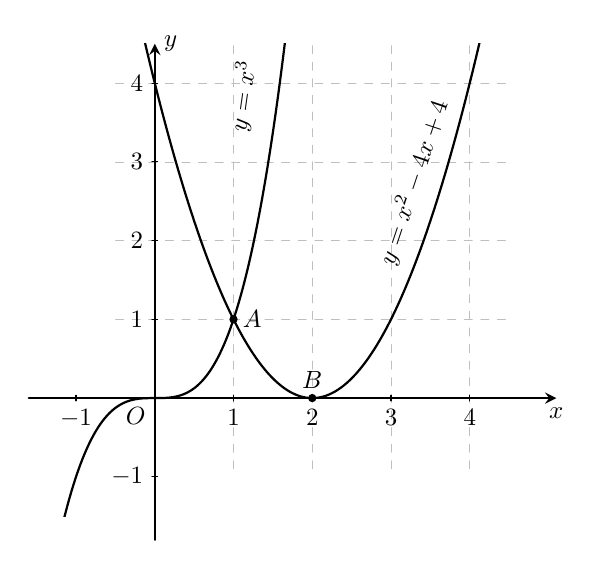
\begin{tikzpicture}[line join=round, line cap=round,>=stealth,thick]
	\tikzset{every node/.style={scale=0.9}}
	\draw[dashed, step=1, gray!50,very thin] (-.5,-0.9) grid (4.5,4.5);
	\draw[->] (-1.6,0)--(5.1,0) node[below] {$x$};
	\draw[->] (0,-1.8)--(0,4.5) node[right] {$y$};
	\draw (0,0) node [below left] {$O$};
	\foreach \x/\nx in {-1/-1,1/1,2/2,3/3,4/4}
	\draw[thin] (\x,1pt)--(\x,-1pt) node [below] {$\nx$};
	\foreach \y/\ny in {-1/-1,1/1,2/2,3/3,4/4}
	\draw[thin] (1pt,\y)--(-1pt,\y) node [left] {$\ny$};
	\begin{scope}
		\clip (-1.5,-1.5) rectangle (4.5,4.5);
		\draw plot[samples=200,domain=-1.2:1.7,smooth,variable=\x] (\x,{(1*(\x)^3});
		\path (1,1)--(2,8) node[pos=0.4,above, sloped]{$y=x^3$};
		\draw plot[samples=200,domain=-0.3:4.3,smooth,variable=\x] (\x,{1*(\x)^2+-4*(\x)+4});
		\path (3,1)--(4,4) node[pos=0.55,above, sloped]{$y=x^2-4x+4$};
		\fill[black](1,1) circle (1.5pt) node[right]{$A$};
		\fill[black](2,0) circle (1.5pt) node[above]{$B$};
	\end{scope}
\end{tikzpicture}
}
\shortans{$1{,}08$}
\loigiai{
	Ta có $V=\pi\displaystyle\int_0^1{\left(x^3\right)^2\mathrm{\,d}x}+\pi\displaystyle\int_1^2{\left(x^2-4x+4\right)^2\mathrm{\,d}x} \approx 1{,}08$.
}
\end{ex}

%Câu 30
\begin{ex}%[2D4V3-3]
\immini{Gọi $V$ là thể tích khối tròn xoay tạo thành khi quay hình phẳng giới hạn bởi các đường $y=\sqrt{x}$, $y=0$ và $x=4$ quanh trục $Ox$. Đường thẳng $x=a$, $\left(0<a<4\right)$ cắt đồ thị hàm số $y=\sqrt{x}$ tại $M$ (hình vẽ). Gọi $V_1$ là thể tích khối tròn xoay tạo thành khi quay tam giác $OMH$ quanh trục $Ox$. Biết rằng $V=2V_1$. Tìm $a$.
}{
\begin{tikzpicture}[line join=round, line cap=round,>=stealth,thick]
	\tikzset{every node/.style={scale=0.9}}
	\draw[->] (-0.6,0)--(5.1,0) node[below left] {$x$};
	\draw[->] (0,-0.4)--(0,2.5) node[below left] {$y$};
	\draw (0,0) node [below left] {$O$};
	\foreach \x/\nx in {3/a,4/4}
	\draw[thin] (\x,1pt)--(\x,-1pt) node [below] {$\nx$};
	\begin{scope}
		\clip (-1.0,-1.0) rectangle (4.5,2.5);
		\draw plot[samples=200,domain=0:4.5,smooth,variable=\x] (\x,{sqrt((\x))});
		\path (0,0)--(4,1) node[pos=0.45,above=0.8cm, sloped]{$y=\sqrt x$};
		\fill[black](3,1.732) circle (1.5pt) node[above right]{$M$} (4,0) node[above right]{$H$};
		\draw (3,2)--(3,-0.1);
		\draw[pattern=north east lines](0,0)--(3,1.732)--(4,0);
	\end{scope}
\end{tikzpicture}
}
\shortans{$3$}
\loigiai{
\immini{
Ta có $V=\pi\displaystyle\int\limits_0^4x\mathrm{\,d}x=\pi\dfrac{x^2}{2}\Bigg|_0^4=8\pi$.\\
Mà $V=2V_1\Rightarrow{V_1}=4\pi$.\\
Gọi $K$ là hình chiếu của $M$ trên $Ox$.\\
Suy ra $OK=a$, $KH=4-a$, $MK=\sqrt a$.\\
Khi xoay tam giác $OMH$ quanh $Ox$ ta được khối
}{
\begin{tikzpicture}[line join=round, line cap=round,>=stealth,thick]
	\tikzset{every node/.style={scale=0.9}}
	\draw[->] (-0.6,0)--(5.1,0) node[below left] {$x$};
	\draw[->] (0,-0.4)--(0,2.5) node[below left] {$y$};
	\draw (0,0) node [below left] {$O$};
	\foreach \x/\nx in {3/a,4/4}
	\draw[thin] (\x,1pt)--(\x,-1pt) node [below] {$\nx$};
	\begin{scope}
		\clip (-1.0,-1.0) rectangle (4.5,2.5);
		\draw plot[samples=200,domain=0:4.5,smooth,variable=\x] (\x,{sqrt((\x))});
		\path (0,0)--(4,1) node[pos=0.45,above=0.8cm, sloped]{$y=\sqrt x$};
		\fill[black](3,1.732) circle (1.5pt) node[above right]{$M$} (4,0) node[above right]{$H$} (3,0)node[below right]{$K$};
		\draw (3,2)--(3,-0.1);
		\draw[pattern=north east lines](0,0)--(3,1.732)--(4,0);
	\end{scope}
\end{tikzpicture}
}\hspace{-0.77cm}
 tròn xoay là sự lắp ghép của hai khối nón sinh bởi các tam giác $OMK$, $MHK$, hai khối nón đó có cùng mặt đáy và có tổng chiều cao là $OH=4$ nên thể tích của khối tròn xoay đó là $V_1=\dfrac{1}{3} \cdot \pi \cdot 4 \cdot \left(\sqrt a\right)^2=\dfrac{4\pi a}{3}$, từ đó suy ra $a=3$.
}
\end{ex}

\Closesolutionfile{ans}
\indapan{6}{ans/ans-2-C4B3CD2_5-10-KQ}

